% По умолчанию используется шрифт 14 размера. Если нужен 12-й шрифт, уберите опцию [14pt]
\documentclass[14pt
  , russian
  %, xcolor={svgnames}
  ]{matmex-diploma-custom}
\usepackage[table]{xcolor}
\usepackage{graphicx}
\usepackage{tabularx}
\newcolumntype{Y}{>{\centering\arraybackslash}X}
\usepackage{amsmath}
\usepackage{amsthm}
\usepackage{amsfonts}
\usepackage{amssymb}
\usepackage{mathtools}
\usepackage{thmtools}
\usepackage{thm-restate}
\usepackage{tikz}
\usepackage{wrapfig}
% \usepackage[kpsewhich,newfloat]{minted}
% \usemintedstyle{vs}
\usepackage[inline]{enumitem}
\usepackage{subcaption}
\usepackage{caption}
\usepackage[nocompress]{cite}
\usepackage{makecell}
% \setitemize{noitemsep,topsep=0pt,parsep=0pt,partopsep=0pt}
% \setenumerate{noitemsep,topsep=0pt,parsep=0pt,partopsep=0pt}


\graphicspath{ {resources/} }

% 
% % \documentclass 
% %   [ a4paper        % (Predefined, but who knows...)
% %   , draft,         % Show bad things.
% %   , 12pt           % Font size.
% %   , pagesize,      % Writes the paper size at special areas in DVI or
% %                    % PDF file. Recommended for use.
% %   , parskip=half   % Paragraphs: noindent + gap.
% %   , numbers=enddot % Pointed numbers.
% %   , BCOR=5mm       % Binding size correction.
% %   , submission
% %   , copyright
% %   , creativecommons 
% %   ]{eptcs}
% % \providecommand{\event}{ML 2018}  % Name of the event you are submitting to
% % \usepackage{breakurl}             % Not needed if you use pdflatex only.
% 
% \usepackage{underscore}           % Only needed if you use pdflatex.
% 
% \usepackage{booktabs}
% \usepackage{amssymb}
% \usepackage{amsmath}
% \usepackage{mathrsfs}
% \usepackage{mathtools}
% \usepackage{multirow}
% \usepackage{indentfirst}
% \usepackage{verbatim}
% \usepackage{amsmath, amssymb}
% \usepackage{graphicx}
% \usepackage{xcolor}
% \usepackage{url}
% \usepackage{stmaryrd}
% \usepackage{xspace}
% \usepackage{comment}
% \usepackage{wrapfig}
% \usepackage[caption=false]{subfig}
% \usepackage{placeins}
% \usepackage{tabularx}
% \usepackage{ragged2e}
% \usepackage{soul}
\usepackage{csquotes}
% \usepackage{inconsolata}
% 
% \usepackage{polyglossia}   % Babel replacement for XeTeX
%   \setdefaultlanguage[spelling=modern]{russian}
%   \setotherlanguage{english}
% \usepackage{fontspec}    % Provides an automatic and unified interface 
%                          % for loading fonts.
% \usepackage{xunicode}    % Generate Unicode chars from accented glyphs.
% \usepackage{xltxtra}     % "Extras" for LaTeX users of XeTeX.
% \usepackage{xecyr}       % Help with Russian.
% 
% %% Fonts
% \defaultfontfeatures{Mapping=tex-text}
% \setmainfont{CMU Serif}
% \setsansfont{CMU Sans Serif}
% \setmonofont{CMU Typewriter Text}

\usepackage[final]{listings}

\lstdefinelanguage{ocaml}{
keywords={@type, function, fun, let, in, match, with, when, class, type,
nonrec, object, method, of, rec, repeat, until, while, not, do, done, as, val, inherit, and,
new, module, sig, deriving, datatype, struct, if, then, else, open, private, virtual, include, success, failure,
lazy, assert, true, false, end},
sensitive=true,
commentstyle=\small\itshape\ttfamily,
keywordstyle=\ttfamily\bfseries, %\underbar,
identifierstyle=\ttfamily,
basewidth={0.5em,0.5em},
columns=fixed,
fontadjust=true,
literate={->}{{$\to$}}3 {===}{{$\equiv$}}1 {=/=}{{$\not\equiv$}}1 {|>}{{$\triangleright$}}3 {\\/}{{$\vee$}}2 {/\\}{{$\wedge$}}2 {>=}{{$\ge$}}1 {<=}{{$\le$}} 1,
morecomment=[s]{(*}{*)}
}

\lstset{
mathescape=true,
%basicstyle=\small,
identifierstyle=\ttfamily,
keywordstyle=\bfseries,
commentstyle=\scriptsize\rmfamily,
basewidth={0.5em,0.5em},
fontadjust=true,
language=ocaml
}
 
\newcommand{\cd}[1]{\texttt{#1}}
\newcommand{\inbr}[1]{\left<#1\right>}


\newcolumntype{L}[1]{>{\raggedright\let\newline\\\arraybackslash\hspace{0pt}}m{#1}}
\newcolumntype{C}[1]{>{\centering\let\newline\\\arraybackslash\hspace{0pt}}m{#1}}
\newcolumntype{R}[1]{>{\raggedleft\let\newline\\\arraybackslash\hspace{0pt}}m{#1}}



\usepackage{soul}
\usepackage[normalem]{ulem}
%\sout{Hello World}

% перевод заголовков в листингах
\renewcommand\lstlistingname{Листинг}
\renewcommand\lstlistlistingname{Листинги}

\usepackage{afterpage}
\usepackage{pdflscape}

\begin{document}
% Титульный лист (ГОСТ Р 7.0.11-2001, 5.1)
\thispagestyle{empty}
\begin{center}
\thesisOrganization
\end{center}
%
\vspace{0pt plus4fill} %число перед fill = кратность относительно некоторого расстояния fill, кусками которого заполнены пустые места
\IfFileExists{images/SPbGU_Logo.png}{
  \begin{minipage}[b]{0.5\linewidth}
    \begin{flushleft}
      
\includegraphics[height=3.5cm]{SPbGU_Logo}
    \end{flushleft}
  \end{minipage}%
  \begin{minipage}[b]{0.5\linewidth}
    \begin{flushright}
      На правах рукописи\\
%      \textsl {УДК \thesisUdk}
    \end{flushright}
  \end{minipage}
}{
\begin{flushright}
На правах рукописи

%\textsl {УДК \thesisUdk}
\end{flushright}
}
%
\vspace{0pt plus6fill} %число перед fill = кратность относительно некоторого расстояния fill, кусками которого заполнены пустые места
\begin{center}
{\large \thesisAuthor}
\end{center}
%
\vspace{0pt plus1fill} %число перед fill = кратность относительно некоторого расстояния fill, кусками которого заполнены пустые места
\begin{center}
\textbf {\large %\MakeUppercase
\thesisTitle}

\vspace{0pt plus2fill} %число перед fill = кратность относительно некоторого расстояния fill, кусками которого заполнены пустые места
{%\small
Специальность \thesisSpecialtyNumber\ "---

<<\thesisSpecialtyTitle>>
}

\ifdefined\thesisSpecialtyTwoNumber
{%\small
Специальность \thesisSpecialtyTwoNumber\ "---

<<\thesisSpecialtyTwoTitle>>
}
\fi

\vspace{0pt plus2fill} %число перед fill = кратность относительно некоторого расстояния fill, кусками которого заполнены пустые места
Диссертация на соискание учёной степени

\thesisDegree
\end{center}
%
\vspace{0pt plus4fill} %число перед fill = кратность относительно некоторого расстояния fill, кусками которого заполнены пустые места
\begin{flushright}
\ifdefined\supervisorTwoFio
Научные руководители:

\supervisorRegalia

\ifdefined\supervisorDead
\framebox{\supervisorFio}
\else
\supervisorFio
\fi

\supervisorTwoRegalia

\ifdefined\supervisorTwoDead
\framebox{\supervisorTwoFio}
\else
\supervisorFio
\fi
\else
Научный руководитель:

\supervisorRegalia

\ifdefined\supervisorDead
\framebox{\supervisorFio}
\else
\supervisorFio
\fi
\fi

\end{flushright}
%
\vspace{0pt plus4fill} %число перед fill = кратность относительно некоторого расстояния fill, кусками которого заполнены пустые места
{\centering\thesisCity\ "--- \thesisYear\par}

\maketitle
\setcounter{tocdepth}{3}
\tableofcontents

% \begin{abstract}
%   В курсаче не нужен
% \end{abstract}

\section{Introduction}


Language-constrained path querying~\cite{barrett2000formal} is a technique for graph navigation querying.
This technique allows one to use formal languages as constraints on paths in edge-labeled graphs: path satisfies constraints if labels along it form a word from the specified language.

The utilization of regular languages as constraints, or \textit{Regular Path Querying} (RPQ), is most well-studied and widespread.
Different aspects of RPQs are actively studied in graph databases~\cite{10.1145/2463664.2465216, 10.1145/3104031,10.1145/2850413}, while regular constraints are supported in such popular query languages as PGQL~\cite{10.1145/2960414.2960421} and SPARQL\footnote{Specification of regular constraints in SPARQL property paths: \url{https://www.w3.org/TR/sparql11-property-paths/}. Access date: 07.07.2020.}~\cite{10.1007/978-3-319-25007-6_1} (property paths).
Nevertheless, there is certainly room for improvement of RPQ efficiency, and new solutions are being created~\cite{Wang2019,10.1145/2949689.2949711}.

At the same time, using more powerful languages, namely context-free languages, as constraints has gained popularity in the last few years.
\textit{Context-Free Path Querying} problem (CFPQ) was introduced by Mihalis Yannakakis in 1990 in~\cite{Yannakakis}.
Many algorithms were proposed since that time, but recently, Jochem Kuijpers et al. showed in~\cite{Kuijpers:2019:ESC:3335783.3335791} that state-of-the-art CFPQ algorithms are not performant enough for practical use.
This motivates us to develop new algorithms for CFPQ.

One promising way to achieve high-performance solutions for graph analysis problems is to reduce them to linear algebra operations.
This way, GraphBLAS~\cite{7761646} API, the description of basic linear algebra primitives, was proposed.
Solutions that use libraries that implement this API, such as SuiteSparce~\cite{10.1145/3322125} and CombBLAS~\cite{10.1177/1094342011403516}, show that reduction to linear algebra is a way to utilize high-performance parallel and distributed computations for graph analysis.

Rustam Azimov shows in~\cite{Azimov:2018:CPQ:3210259.3210264} how to reduce CFPQ to matrix multiplication.
Later, it was shown in~\cite{Mishin:2019:ECP:3327964.3328503} and~\cite{10.1145/3398682.3399163} that utilization of appropriate libraries for linear algebra for Azimov's algorithm implementation makes a practical solution for CFPQ.
However Azimov's algorithm requires transforming the input grammar to Chomsky Normal Form, which leads to the grammar size increase, and hence worsens performance, especially for regular queries and complex context-free queries.

To solve these problems, an algorithm based on automata intersection was proposed~\cite{10.1007/978-3-030-54832-2_6}.
This algorithm is based on linear algebra and does not require the transformation of the input grammar.
We improve the algorithm in this work.
We reduce the above mentioned solution to operations over Boolean matrices, thus simplifying its description and implementation.
Also, we show that this algorithm is performant enough for regular queries, so it is a good candidate for integration with real-world query languages: one algorithm can be used to evaluate both regular and context-free queries.

Moreover, we show that this algorithm opens the way to tackle a long-standing problem about the existence of truly-subcubic $O(n^{3-\epsilon})$ CFPQ algorithm ~\cite{10.1145/1328438.1328460, Yannakakis}.
Currently, the best result is an $O(n^3/\log{n})$ algorithm of Swarat Chaudhuri~\cite{10.1145/1328438.1328460}.
Also, there exist truly subcubic solutions which use fast matrix multiplication for some fixed subclasses of context-free languages~\cite{8249039}.
Unfortunately, this solutions cannot be generalized to arbitrary CFPQs.
In this work, we identify incremental transitive closure as a bottleneck on the way to achieve subcubic time complexity for CFPQ.

To sum up, we make the following contributions.
\begin{enumerate}
	\item We rethink and improve the CFPQ algorithm based on tensor-product proposed by Orachev et al. ~\cite{10.1007/978-3-030-54832-2_6}.
	We reduce this algorithm to operations over Boolean matrices.
	As a result, all-path query semantics is handled, as opposed to the previous matrix-based solution which handles only the single-path semantics.
	Also, both regular and context-free grammars can be used as queries.
	We prove the correctness and time complexity for the proposed algorithm.
	\item We demonstrate the interconnection between CFPQ and incremental transitive closure.
	We show that incremental transitive closure is a bottleneck on the way to achieve faster CFPQ algorithm for general case of arbitrary graphs as well as for special families of graphs, such as planar graphs.
	\item We implement the described algorithm and evaluate it on real-world data for both RPQ and CFPQ. Results show that the proposed solution is comparable with existing solutions for CFPQ and RPQ, thus it is a promising way to create a unified algorithm for both CFPQ and RPQ evaluation.
\end{enumerate}
\section{Цель и задачи}

Целью данной работы является реализация алгоритма поиска путей в графовых базах данных через тензорное произведение на GPGPU. Для ее выполнения были поставлены следующие задачи.

\begin{itemize}
    \item Разработка архитектуры библиотеки примитивов разреженной линейной булевой алгебры для вычислений на GPGPU.
    \item Реализация библиотеки в соответствии с разработанной архитектурой.
    \item Реализация алгоритма поиска путей с КС ограничениями через тензорное произведение с использованием разработанной библиотеки.
    \item Экспериментальное исследование библиотеки и реализации алгоритма.
\end{itemize}
\section{Обзор предметной области}

Для разработки библиотеки и реализации нового алгоритма необходимо сперва рассмотреть базовую теорию запросов к графам с КС ограничениями, а также ознакомиться с существующими подходами к реализации.
Для этого предлагается рассмотреть алгоритмы выполнения данных запросов, с акцентом на перспективное направление алгоритмов, которые полагаются на операции разреженной линейной алгебры. Необходимо рассмотреть алгоритм поиска путей на основе тензорного произведения, а также существующие инструменты для работы с примитивами разреженной линейной алгебры на GPU. Это поможет обосновать необходимость разработки нового подобного инструмента.

\subsection{Терминология}

% В этой секции изложены основные определения и факты из теории графов и формальных языков, необходимые для понимания предметной области. 
    
\textit{Ориентированный граф с метками на ребрах} $\mathcal{G} = \langle V, E, L \rangle$ это тройка объектов, где $V$ конечное непустое множество вершин графа, $E \subseteq V \times L \times V$ конечное множество ребер графа, $L$ конечное множество меток графа. Здесь и далее будем считать, что вершины графа индексируются целыми числами, т.е. $V = \{0~,...,~|V| - 1\}$.

Граф $\mathcal{G} = \langle V, E, L \rangle$ можно представить в виде матрицы смежности $M$ размером $|V| \times |V|$, где $M[i,j] = \{l~|~(i,l,j) \in E\}$. Используя булеву матричную декомпозицию, можно представить матрицу смежности в виде набора матриц $\mathcal{M} = \{ M^l ~|~ l \in L, M^l[i,j] = 1 \iff l \in M[i,j]\}$.

Путь $\pi$ в графе $\mathcal{G} = \langle V, E, L \rangle$ это последовательность ребер $e_0,e_1,e_{n-1}$, где $e_i = (v_i, l_i, u_i) \in E$ и для любых $e_i, e_{i+1}: u_i = v_{i+1}$. Путь между вершинами $v$ и $u$ будем обозначать как $v \pi u$. Слово, которое формирует путь $\pi = (v_0, l_0, v_1), ... ,(v_{n-1}, l_{n-1}, v_n)$ будем обозначать как $\omega (\pi) = l_0 ... l_{n-1}$, что является конкатенацией меток вдоль этого пути $\pi$.

\textit{Контекстно-свободная (КС) грамматика} $G = \langle \Sigma, N, P, S \rangle$ это четверка объектов, где $\Sigma$ конечное множестве терминалов или терминальный алфавит, $N$ конечное множество нетерминалов, $P$ конечное множество правил вывода вида $A \rightarrow \gamma, \gamma \in (N \cup \Sigma)^*$, $S \in N$ стартовый нетерминал. Вывод слова $w$ в грамматике из нетерминала $S$ применением одного или нескольких правил вывода обозначается как $S \rightarrow^*_G w$.

Язык $\mathcal{L}$ над конечным алфавитом символов $\Sigma$ --- множество слов, составленных из символов этого алфавита, т.е. $\mathcal{L} \subseteq \{w~|~w \in \Sigma ^*\}$. Язык, задаваемый грамматикой $G$, обозначим как $\mathcal{L}(G) = \{w~|~S \rightarrow^*_G w\}$.

\textit{Произведение Кронекера} матриц $A$ и $B$ с размером $m \times n$ и $p \times q$ соответственно это блочная матрица размера $mp \times nq$, где блок с индексом $(i,j)$ вычисляется как $a_{ij} * B$.

% Keep this thing commented
% \begin{figure}[h]
%     \centering
%     \begin{subfigure}[b]{0.50\textwidth}
%         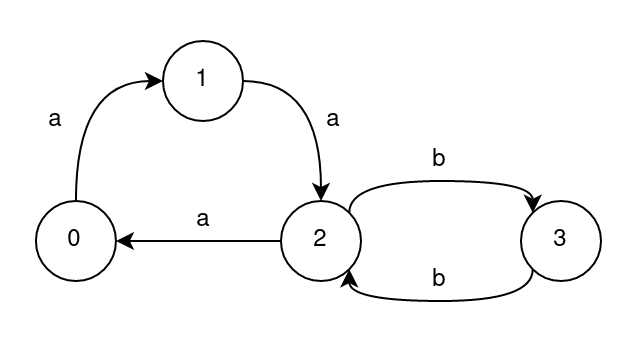
\includegraphics[width=\textwidth]{images/example_graph.png}
%         \caption{Ориентированный граф с меткам}
%     \end{subfigure}
%     \hfill
%     \begin{subfigure}[b]{0.20\textwidth}
%         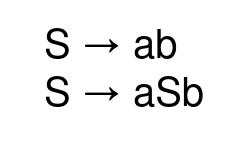
\includegraphics[width=\textwidth]{images/exmample_grammar.png}
%         \caption{Грамматика}
%     \end{subfigure}
%     \caption{Пример графа и грамматики}
% \end{figure}

\subsection{Поиск путей с ограничениями}

При вычислении запроса на поиск путей в графе $\mathcal{G} = \langle V, E, L \rangle$ в качестве ограничения выступает некоторый язык $\mathcal{L}$, которому должны удовлетворять результирующие пути.

Поиск путей в графе с семантикой \textbf{достижимости} --- это поиск всех таких пар вершин $(v,u)$, что между ними существует путь $v \pi u$ такой, что $\omega (\pi) \in \mathcal{L}$. Результат запроса обозначается как $R = \{ (v,u)~|~\exists v \pi u : \omega (\pi) \in \mathcal{L} \}$.

Поиск путей в графе с семантикой \textbf{всех путей} --- это поиск всех таких путей $v \pi u$,   что $\omega (\pi) \in \mathcal{L}$. Результат запроса обозначается как $\Pi = \{ v \pi u~|~v \pi u : \omega (\pi) \in \mathcal{L} \}$.
Необходимо отметить, что множество $\Pi$ может быть бесконечным, поэтому в качестве результата запроса предполагается не всё множество в явном виде, а некоторый \textit{итератор}, который позволит последовательно извлекать все пути.

Семантика \textbf{одного пути} является ослабленной формулировкой семантики всех путей, так как для получения результата достаточно найти всего один путь вида $v \pi u : \omega (\pi) \in \mathcal{L}$ для каждой пары $(v, u) \in R$.

Поскольку язык $\mathcal{L}$ может быть бесконечным, при составлении запросов используют не множество $\mathcal{L}$ в явном виде, а некоторое правило формирования слов этого языка. В качестве таких правил и выступают регулярные выражения или КС грамматики. При именовании запросов отталкиваются от типа правил, поэтому запросы именуются как регулярные или КС соответственно.

\subsection{Существующие решения}

Впервые проблема выполнения запросов с контекстно-свободными ограничениями была сформулирована в 1990 году в работе Михалиса Яннакакиса~\cite{inproceedings:yannakakis_cfpq_problem}. С того времени были представлены многие работы, в которых так или иначе предлагалось решение данной проблемы. 

Однако недавно  Йохем Куиджперс и др.~\cite{article:kuijpers_cfpq_exp_compare} на основе сравнения нескольких алгоритмов~\cite{article:hellings_cfpq,inproceedings:matrix_cfpq,inbook:santos_cfpq_lr_analysis} для выполнения запросов с контекстно-свободными ограничениями заключили, что существующие алгоритмы неприменимы для практики из-за проблем с производительностью.
Стоит отметить, что алгоритмы, используемые в статье, были реализованы на языке программирования \textit{Java} и исполнялись в среде \textit{JVM} в однопоточном режиме, что могло существенно повлиять на производительность представленных алгоритмов и, соответственно, выводы авторов.

Это подтверждают результаты работы Арсения Терехова и др.~\cite{inproceedings:cfqp_matrix_with_single_source}, в которой с использованием программных и аппаратных средств Nvidia Cuda был реализован алгоритм Рустама Азимова~\cite{inproceedings:matrix_cfpq}. В данном алгоритме задача поиска путей с КС ограничениями была сведена к операциям линейной алгебры, что позволило использовать высокопроизводительные библиотеки для выполнения данных операций на GPGPU. 
Данное исследование показало, что эффективная реализация алгоритма на GPU может сделать его применимым для анализа реальных данных.


Алгоритм Рустама Азимова~\cite{inproceedings:cfqp_matrix_with_single_source} способен выполнять запросы только в семантике одного пути. Поскольку в качестве формализма для представления грамматики КС запроса используется \textit{ослабленная нормальная форма Хомского (ОНФХ)}~\cite{book:automata_theory}, увеличение числа правил в исходной грамматике запроса может приводить к существенному разрастанию ОНФХ, что негативно влияет на время работы алгоритма.

\subsection{Поиск путей с КС ограничениями через тензорное произведение}

Представленный в работе Егора Орачева и др.~\cite{inbook:kronecker_cfpq_adbis} алгоритм для выполнения КС запросов использует операции линейной булевой алгебры: произведение Кронекера (частный случай тензорного произведения), матричное умножение и сложение. Данный алгоритм позволяет выполнять запросы в семантике достижимости и всех путей, а также он подходит для реализации на многоядерных системах, что делает его потенциально применимым для анализа реальных данных. Кроме этого, данный алгоритм использует в качестве формализма для представления запроса \textit{рекурсивный автомат} (РА)~\cite{article:recursive_state_machines}, что потенциально может решить проблему разрастания исходной грамматики запроса. 

Идея алгоритма состоит в \textit{пересечении} РА и графа с использованием некоторой модификации классического алгоритма пересечения конечных автоматов~\cite{book:automata_theory}. Пересечение выполняется с использованием произведения Кронекера, а множество рекурсивных вызовов учитывается с помощью транзитивного замыкания, что также выражается с использованием матричных операций умножения и поэлементного сложения. Данный процесс итеративный, и он выполняется до тех пор, пока в результирующий граф добавляются новые ребра.

% Далее предлагается рассмотреть описание данного алгоритма и используемую им технику сведения вычислений к операциям линейной алгебры.

% \subsubsection*{Рекурсивный автомат}

% Для представления входной грамматики КС запроса алгоритм~\cite{inbook:kronecker_cfpq_adbis} использует \textit{рекурсивный автомат}. Данный формализм является своего рода обобщением \textit{недетерминированного конечного автомата} на случай КС языков. Для понимания того, как он устроен, обратимся к теории формальных языков.

% \textit{Недетерминированный конечный автомат} (НКА) $F = \langle \Sigma, Q, Q_s, Q_f, \delta \rangle$ это пятерка объектов, где:

% \begin{itemize}
%     \item $\Sigma$ конечное множество входных символов или алфавит
%     \item $Q$ конечное множество состояний
%     \item $Q_s \subseteq Q$ множество стартовых состояний
%     \item $Q_f \subseteq Q$ множество конечных состояний
%     \item $\delta : \Sigma \times Q \rightarrow 2^Q$ функция переходов автомата
% \end{itemize}

% Язык, допускаемый автоматом $F$ будем обозначать как $L(F)$. Любое регулярное выражение может быть преобразовано в соответствующий НКА~\cite{book:automata_theory}. 

% \textit{Рекурсивный автомат} (РА) $R = \langle M, m, \{C_i\}_{i \in M} \rangle$ это тройка объектов, где: 

% \begin{itemize}
%     \item $M$ конечное множество меток компонентных НКА, называемых далее \textit{модули}
%     \item $m$ метка стартового модуля
%     \item $\{C_i\}$ множество модулей, где модуль $C_i = \langle \Sigma \cup M, Q_i, S_i, F_i, \delta _i \rangle$ состоит из:
%     {
%     \begin{itemize}
%         \item $\Sigma \cup M$ множество символов модуля, $\Sigma \cap M = \emptyset$
%         \item $Q_i$ конечное множество состояний модуля, $Q_i \cap Q_j = \emptyset, \forall i \neq j$
%         \item $S_i \subseteq Q_i$ множество стартовых состояний модуля
%         \item $F_i \subseteq Q_i$ множество конечных состояний модуля 
%         \item $\delta_i : (\Sigma \cup M) \times Q_i \rightarrow 2^{Q_i}$ функция переходов
%     \end{itemize}
%     }
% \end{itemize}

% Рекурсивный автомат ведет себя как набор НКА или модулей~\cite{article:recursive_state_machines}. Эти модули очень сходны с НКА при обработке входных последовательностей символов, однако они способны обрабатывать дополнительные \textit{рекурсивные вызовы} за счет неявного \textit{стека вызовов}, который присутствует во время работы РА. С точки зрения прикладного программиста это похоже на рекурсивные вызовы одних функций из других с той разницей, что вместо функций здесь выступают модули РА.

% Рекурсивные автоматы по своей вычислительной мощности эквивалентны магазинным автоматам~\cite{article:recursive_state_machines}. А поскольку подобный магазинный автомат способен распознавать КС грамматику~\cite{book:automata_theory}, рекурсивные автоматы эквивалентны КС грамматикам. Это позволяет корректно использовать РА для представления входной КС грамматики запроса.

% \subsubsection*{Пересечение рекурсивного автомата и графа}

% Классический алгоритм~\cite{book:automata_theory} \textit{пересечения} двух НКА $F^1$ и $F^2$ позволяет построить новый НКА $F$ с таким свойством, что он допускает пересечение исходных регулярных языков, т.е. $L(F) = L(F^1) \cap L(F^2)$. Формально, для $F^1 = \langle \Sigma, Q^1, Q^1_S, Q^1_F, \delta^1 \rangle$ и $F^2 = \langle \Sigma, Q^2, Q^2_S, Q^2_F, \delta^2 \rangle$ строится новый НКА $F = \langle \Sigma, Q, Q_S, Q_F, \delta \rangle$, где:

% \begin{itemize}
%     \item $Q = Q^1 \times Q^2$
%     \item $Q_S = Q^1_S \times Q^2_S$
%     \item $Q_F = Q^1_F \times Q^2_F$
%     \item $\delta: \Sigma \times Q \rightarrow Q$ и $\delta(s, \langle q_1, q_2 \rangle) = \langle q'_1, q'_2 \rangle$, если $\delta^1 (s, q_1)=q'_1$ и $\delta^2 (s, q_2)=q'_2$ 
% \end{itemize}

% Интерпретируя ориентированный граф с метками как некоторый конечный автомат, в котором все вершины графа являются одновременно начальными и конечными состояниями автомата, а ребра графа --- переходами между состояниями автомата, возможно пересечь этот граф и некоторый НКА, используя алгоритм пересечения, описанный выше. Однако, если представить граф и функцию переходов КА, тоже интерпретируемую как граф, в виде матриц смежности, можно использовать \textit{произведение Кронекера} для построения функции переходов автомата пересечения.

% \textit{Произведение Кронекера} для двух матриц $A$ и $B$ размера $m_1 \times n_1$ и $m_2 \times n_2$ с поэлементной операцией умножения $\cdot$ дает матрицу $M = A \otimes B$ размером $m_1 * m_2 \times n_1 * n_2$, где $M[u * m_2 + v, p * n_2 + q] = A[u, p] \cdot B[v, q]$. 

% Поскольку РА состоит из набора модулей, которые по своей структуре не сильно отличаются от классических НКА, это дает идею для применения похожего алгоритма пересечения РА и графа, с той  разницей, что процесс пересечения будет итеративным и будет включать в себя транзитивное замыкание, чтобы учесть \textit{рекурсивные вызовы}, присутствующие в РА. 

% \subsubsection*{Описание алгоритма}

В листинге~\ref{tensor:cfpq} представлен псевдокод алгоритма. Необходимо отметить, что алгоритм использует булеву матричную декомпозицию в строках \textbf{3 -- 4} для представления матрицы переходов РА и матрицы смежности графа, а также использует матричное умножение, сложение и произведение Кронекера в строках \textbf{14 -- 16}.

Данный алгоритм является относительно простым в реализации, так как всю сложность выполнения он перекладывает на операции линейной алгебры, которые должны быть реализованы в сторонних высокопроизводительных библиотеках.

\begin{algorithm}[h]
\floatname{algorithm}{Listing}
\begin{algorithmic}[1]
\footnotesize
\caption{Поиск путей через произведение Кронекера}
\label{tensor:cfpq}
\Function{KroneckerProductBasedCFPQ}{G, $\mathcal{G}$}
    % Input data preparation
    \State{$R \gets$ Рекурсивный автомат для грамматики $G$}
    \State{$\mathcal{M}_1 \gets$ Матрица переходов $R$ в булевой форме}
    \State{$\mathcal{M}_2 \gets$ Матрица смежности $\mathcal{G}$ в булевой форме}
    \State{$C_3 \gets$ Пустая матрица}
    % Eps-transition handling for graph
    \For{$s \in \{0,...,dim(\mathcal{M}_1)-1\}$}
        \For{$S \in \textit{getNonterminals}(R,s,s)$}
            \For{$i \in \{0,...,dim(\mathcal{M}_2)-1\}$}
                % Or just $M_2^n[i,i] \gets M_2^n[i,i] \vee \{1\}$ ??? 
                \State{$M_2^S[i,i] \gets \{1\}$}
            \EndFor
        \EndFor
    \EndFor
    \While{Матрица смежности $\mathcal{M}_2$ изменяется}
        % Kronecker product (i.e. partial intersection)
        \State{$\mathcal{M}_3 \gets \mathcal{M}_1 \otimes \mathcal{M}_2$}
        \Comment{Вычисление произведения Кронекера}
        % Collapse to single Boolean matrix
        \State{$M'_3 \gets \bigoplus_{M_3^a \in \mathcal{M}_3} M_3^a $}
        \Comment{Слияние матриц в одну булеву матрицу достижимости}
        % Closure over Boolean matrix only
        \State{$C_3 \gets \textit{transitiveClosure}(M'_3)$}
        \Comment{Транзитивное замыкание для учета рекурсивных вызовов}
        \State{$n \times n \gets$ dim($M_3)$}
        % Add non-terminals (possibly new)
        \For{$(i,j)~|~C_3[i,j] \neq 0$}
            \State{$s, f \gets \textit{getStates}(C_3,i,j)$}
            \State{$x, y \gets \textit{getCoordinates}(C_3,i,j)$}
            \For{$S \in \textit{getNonterminals}(R,s,f)$}
                \State{$M_2^S[x,y] \gets \{1\}$}
            \EndFor
        \EndFor
    \EndWhile
\State \Return $\mathcal{M}_2,C_3$
\EndFunction
\end{algorithmic}
\end{algorithm}

% Keep this thing commented
% \begin{algorithm}[]
% \floatname{algorithm}{Listing}
% \begin{algorithmic}[1]
% \footnotesize
% \caption{Вспомогательные функции для алгоритма поиска путей}
% \label{tensor:cfpq:help}
% \Function{GetStates}{$C, i, j$}
%     \State{$r \gets dim(\mathcal{M}_1)$}
%     \Comment{$\mathcal{M}_1$ матрица переходов в булевой форме для $R$}
%     \State \Return{$\left\lfloor{i / r}\right\rfloor, \left\lfloor{j / r}\right\rfloor$}
% \EndFunction
% \Function{GetCoordinates}{$C, i, j$}
%     \State{$n \gets dim(\mathcal{M}_2)$}
%     \Comment{$\mathcal{M}_2$ матрица смежности в булевой форме для $\mathcal{G}$}
%     \State \Return{$i \bmod n, j \bmod n$}
% \EndFunction
% \end{algorithmic}
% \end{algorithm}

% todo: paths extraction algorithm
% \subsection{Извлечение всех путей}

\subsection{Вычисления на GPGPU}

\textit{GPGPU} (от англ. General-purpose computing on graphics processing units) --- техника использования графического процессора видеокарты компьютера для осуществления неспециализированных вычислений, 
которые обычно проводит центральный процессор. 
Данная техника позволяет получить значительной прирост производительности в SIMD (англ. single instruction, multiple data) вычислениях, 
когда необходимо обрабатывать большие массивы однотипных данных с фиксированным набором команд.

Исторически видеокарты в первую очередь использовались как графические ускорители для создания высококачественной трехмерной графики в режиме реального времени. Позже стало ясно, что мощность графического процессора можно использовать не только для графических вычислений. Так появились программируемые вычислительные блоки (англ. compute shaders), которые позволяют выполнять на видеокарте неграфические вычисления.

На данный момент существует несколько промышленных стандартов для создания программ, использующих графический процессор, одними из которых являются Vulkan~\cite{net:spec_vulkan}, OpenGL~\cite{net:spec_opengl}, DirectX~\cite{net:spec_direct3d} как API для графических и неспециализированных вычислительных задач, а также OpenCL~\cite{net:spec_opencl}, Nvidia Cuda~\cite{net:cuda_toolkit_docs} как API для неспециализированных вычислений. 

В качестве технологии для GPGPU в этой работе используется Nvidia Cuda. В то время как OpenCL создавался как кросс-платформенный стандарт для программирования вычислений, Cuda API специфичен только для видеокарт производства компании Nvidia. Однако он имеет более широкий набор инструментов как для написания, так и для отладки программ, а также собственный компилятор NVCC, который позволяет осуществлять кросс-компиляцию кода на языке Cuda C/C++, и прозрачно использовать его вместе с кодом на языке C/C++. Кроме этого, в данной работе используются результаты исследования Арсения Терехова и др.~\cite{inproceedings:cfqp_matrix_with_single_source}, в котором также использовался Cuda API.

\subsection{Примитивы разреженной линейной алгебры для GPGPU}

Для эффективной реализации алгоритмов~\cite{inbook:kronecker_cfpq_adbis, inproceedings:matrix_cfpq} требуются высокопроизводительные библиотеки операций линейной алгебры. 
Реальные графовые данные насчитывают порядка $10^5$ -- $10^9$ вершин и являются сильно разреженными, т.е. количество ребер в графе сравнимо с количеством вершин, поэтому плотные матрицы не подходят для представления такого типа данных. К примеру, плотная матрица смежности ориентированного графа без меток с 1000000 вершин, вне зависимости от количества ребер, занимает порядка 116 GB памяти, что является избыточным.

% В качестве такой библиотеки для выполнения матричных операций на центральном процессоре авторы исследований~\cite{inbook:kronecker_cfpq_adbis, inproceedings:cfqp_matrix_with_single_source} использовали \textit{SuiteSparse}~\cite{article:suite_sparse_for_graph_problems}. Это эталонная реализация стандарта \textit{GraphBLAS}~\cite{paper:graphblas_foundations}, который был разработан как некоторый инструмент для реализации алгоритмов обработки графов на языке линейной алгебры.  

% Экспериментальное исследование~\cite{inproceedings:cfpq_matrix_evaluation} по реализации алгоритма Рустама Азимова~\cite{inproceedings:matrix_cfpq} на GPGPU с использованием операций над плотными булевыми матрицами показало, что вычисление на графическом процессоре дает значительный прирост производительности при обработке синтетических данных и данных среднего размера. Однако реальные графовые данные насчитывают порядка $10^5$ -- $10^9$ вершин и являются сильно разреженными, т.е. количество ребер в графе сравнимо с количеством вершин, поэтому плотные матрицы не подходят для представления такого типа данных. 

Библиотеки \textit{cuSPARSE}~\cite{net:cusparse_docs} и \textit{CUSP}~\cite{net:cusplibrary} для платформы Nvidia Cuda и \textit{clSPARSE}~\cite{10.1145/2909437.2909442} для платформы OpenCL предоставляют функциональность для работы с разреженными данными, однако они фокусируются на обработке численных данных и специализируются только на стандартных типах, таких как \textit{float}, \textit{double}, \textit{int} и \textit{long}. Для реализации алгоритмов~\cite{inbook:kronecker_cfpq_adbis, inproceedings:matrix_cfpq} требуются операции над разреженными булевыми матрицами, поэтому требуется специализация вышеуказанных библиотек для работы с булевыми примитивами. С одной стороны, библиотека cuSPARSE имеет закрытый исходный код, что делает невозможным ее модификацию, с другой стороны, библиотеки CUSP и clSPARSE имеет открытый исходный код и свободную лицензию, однако используемые ими алгоритмы умножения разреженных матриц \textit{достаточно} требовательны к ресурсам памяти~\cite{inproceedings:cfqp_matrix_with_single_source}, что делает их неприменимым для обработки данных большого размера.

Также необходимо отметить такие библиотеки как \textit{GraphBLAST}~\cite{yang2019graphblast} и \textit{bhSPARSE}~\cite{10.1016/j.jpdc.2015.06.010}. GraphBLAST является попыткой реализовать стандарт GraphBLAS~\cite{paper:graphblas_foundations} --- промышленный API для анализа графов в терминах линейной алгебры. Данный стандарт позволят использовать произвольные полукольца для вычислений, включая булево полукольцо. bhSPARSE предоставляет реализацию примитивов разреженной линейной алгебры для вычислений в гетерогенных системах, включая GPU. Он также, как и cuSPARSE, CUSP или clSPARSE фокусируется на численных типах данных. GraphBLAST и bhSPARSE находятся в данный момент в активной разработке, поэтому пока что невозможно использовать ни один из инструментов для практических задач.

В работе Арсения Терехова и др.~\cite{inproceedings:cfqp_matrix_with_single_source} была предпринята попытка самостоятеьно реализовать алгоритм умножения разреженных матриц \textit{Nsparse}, предложенный в работе Юсуке Нагасака и др.~\cite{inproceedings:spgemm_mem_saving_for_nvidia}, и специализировать его для булевых значений. Данный алгоритм эксплуатирует возможности видеокарт Nvidia и засчет б\'ольшего количества шагов обработки позволяет снизить количество расходуемой видеопамяти. Эксперименты показали, что подобный подход позволяет не только снизить в разы количество расходуемой видеопамяти, но и снизить общее время работы алгоритма Рустама Азимова~\cite{inproceedings:matrix_cfpq} по сравнению с его реализацией на основе библиотеки \textit{CUSP}. 

% Поэтому было принято решение расширить реализацию матричных операций из работы~\cite{inproceedings:cfqp_matrix_with_single_source}, дополнив ее требуемыми для алгоритма~\cite{inbook:kronecker_cfpq_adbis} примитивами, и оформить решение в виде самостоятельной библиотеки, которая позволила бы в дальнейшем решать сходные вычислительные задачи.

\begin{frame}[fragile]
	\transwipe[direction=90]
	\frametitle{\faCogs\ Модернизация архитектуры}
	
	\begin{columns}
        \begin{column}{0.5\textwidth}
            \begin{figure}[hbt!]{\textwidth}
				\centering
				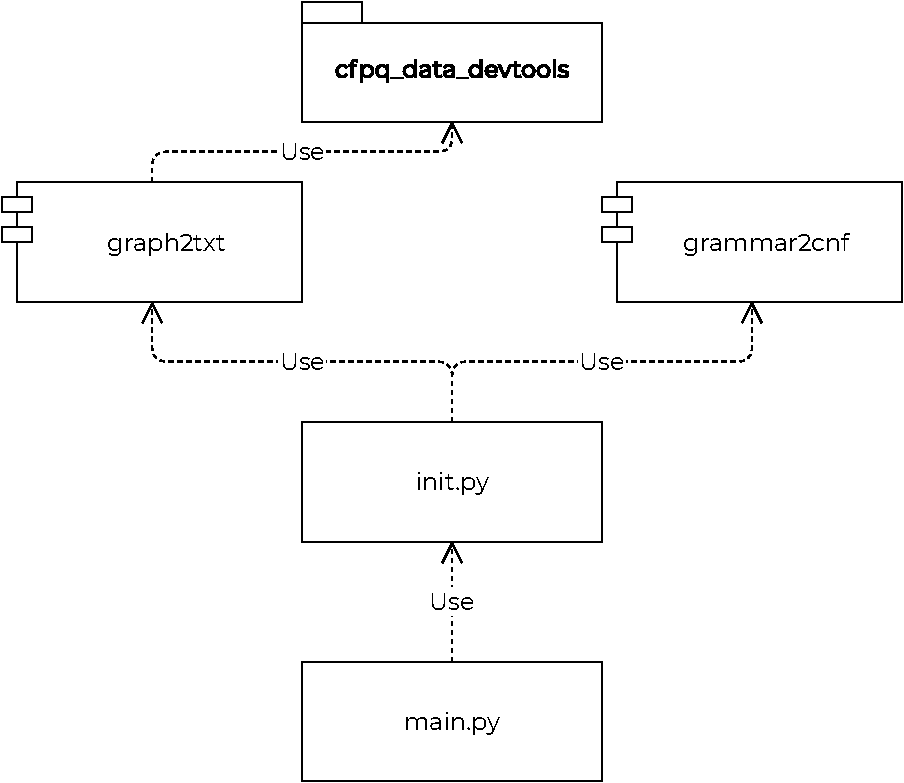
\includegraphics[width=0.9\textwidth]{img/architecture_old.pdf}
				\caption*{Рис. 3. Архитектура <<до>>} \label{fig:architecture_old}
			\end{figure}
        \end{column}

        \begin{column}{0.5\textwidth}
            \begin{figure}[hbt!]{\textwidth}
				\centering
				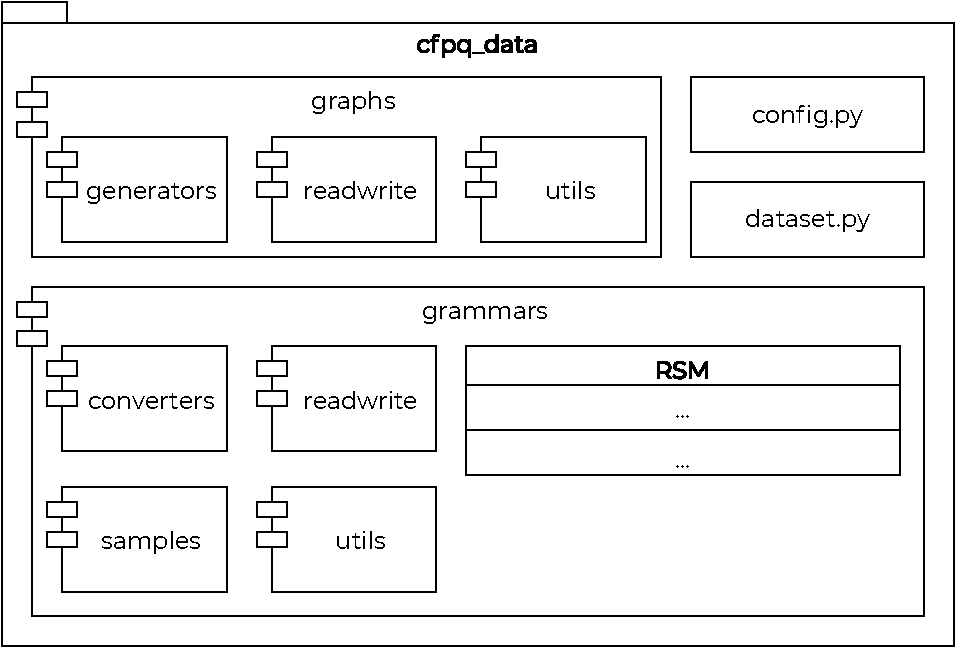
\includegraphics[width=0.9\textwidth]{img/architecture_new.pdf}
				\caption*{Рис. 4. Архитектура <<после>>} \label{fig:architecture_new}
			\end{figure}
        \end{column}
    \end{columns}
\end{frame}

\section{Implementation Details}

In this section we discuss the particular implementation details of the proposed libraries. Although general and architectural specifics are similar, the actual internal storage formats and algorithms are different. With this development strategy we address the potential problem of processing the sparse data with different values distribution, as well as the problem of proper balancing between time of the execution and memory consumption. 

\subsection{cuBool}

cuBool is sparse boolean linear algebra implementation specifically for NVIDIA Cuda platform. Core of this 
library relies on Cuda C/C++ language and API, what with NVCC compiler allows intermix C++ with Cuda 
specifics. Also cuBool employs NVIDIA Thrust auxiliary library, which provides 
implementation for generic data containers and operations, such as \textit{iterating}, \textit{exclusive or 
inclusive scan}, \textit{map} and etc., which are executed on Cuda device. That allows express algorithms in 
terms of high-level optimised primitives, what increases code readability and reduces time for development.

Sparse matrix primitive is stored in the \textit{compressed sparse row} (CSR) format with only two arrays: 
$rowspt$ for row offset indices and $cols$ for columns indices. Boolean matrices has no actual values, thus 
$true$ values are encoded only as $(i, j)$ pairs. It allows to store matrix $M$ of size $m \times n$ 
in $(m + \textit{NNZ(M)}) \times \textit{sizeof(IndexType)}$ bytes of GPU memory, where 
\textit{IndexType} is type of stored indices, for simplicity can be selected as \textit{uint32\_t}.

The algorithm Nspasrse~\cite{inproceedings:cfpq_for_redis_graph} is used for matrix-matrix multiplication. 
This algorithm is a boolean values case 
adaptation of the state-of-the-art, efficient and memory saving sparse general matrix multiplication (SpGEMM) 
algorithm, proposed in Yusuke Nagasaka et al. research~\cite{algo:spgemm:8025284}. This algorithm was selected because it 
gives promising relatively small memory footprint for large matrices processing, as well as it competes with 
other major Cuda SpGEMM implementations, such as cuSPARSE or CUSP.  

Matrix-matrix addition is based on GPU Merge Path algorithm~\cite{inproceedings:gpu_merge_path} with 
dynamic work balancing and two pass processing. 
These optimizations give better workload dispatch among execution blocks and allow more precise memory allocations in
order to keep memory footprint small respectively. 

As an example of library C API embedding, cuBool provides python wrapper, called Pycubool. This module exports 
library functionality via default CTypes module for native functions calling and provides safe and automated 
management for native resources. 

\subsection{clBool}

clBool is sparse boolean linear algebra implementation for OpenCL platform. This library is implemented 
in the C++ with OpenCL kernels, stored as separate source files, loaded on demand at runtime. 

Sparse matrix primitive is stored in \textit{coordinate format} (COO) with two arrays: $rows$ and $cols$ 
for row and column indices of the stored non-zero values. For the matrix $M$ of size $m \times n$ memory 
consumption is $2 \times \textit{NNZ(M)} \times \textit{sizeof(IndexType)}$. This format was selected 
instead of CSR, because COO gives better memory footprint for very sparse matrices with a lot of empty rows.

\textbf{!!! Matrix-matrix multiplication !!!}

Matrix-matrix addition is based on GPU Merge Path algorithm as well. Since all COO matrix values are stored in 
the single array, its merge can be completed at single time, compared to CSR matrix merge computed on a 
per row basis. This operation is implemented in a classic one pass fashion: it allocates single merge 
buffer of size $\textit{NNZ(A)} + \textit{NNZ(B)})$ before actual merge of matrices $A$ and $B$, what can
negatively affect memory consumption for large matrices with lots of duplicated non-zero values at the 
same positions.

\textbf{!!! Something about managed environment wrapper !!!}

\section{Алгоритм поиска путей с КС ограничениями}
\label{section:algo_impl}

В данной секции предлагается рассмотреть основные детали реализации алгоритма~\cite{inbook:kronecker_cfpq_adbis} поиска путей с КС ограничениями через тензорное произведение на GPU с использованием библиотеки cuBool, особенности реализации которой были представлены в предыдущей главе..

Реализация алгоритма написана на языке Python с использованием пакета \textbf{pycubool}.
Программа, исполняемая Python-интерпретатором, задает только последовательность вызовов операций.
Вычислительно-интенсивные части алгоритма выполняются на GPU в рамках библиотеки, 
поэтому решение в целом остается производительным.
 
На вход алгоритм получает граф и КС грамматику. 
Граф представлен в виде булевой матричной декомпозиции матрицы смежности графа.
КС грамматика закодирована в виде рекурсивного автомата. 
Его матрица переходов также представлена в булевой матричной декомпозиции.
На выходе алгоритм возвращает матрицу смежности графа достижимости, а также индекс, 
который позволяет восстанавливать все пути в графе в соответствии с входной грамматикой.

Также с использованием \textbf{pycubool} реализован классический матричный алгоритм Рустама Азимова~\cite{inproceedings:matrix_cfpq}, требуемый для корректного сравнения производительности с алгоритмом на основе тензорного произведения.

Реализации упомянутых алгоритмов доступны в рамках открытого проекта \textbf{CFPQ-PyAlgo}~\cite{net:cfpq_py_algo}.
Данный проект предоставляет инфраструктуру для осуществления замеров производительности, а также для загрузки и конвертации данных, требуемых для экспериментов.
Архитектура данного стенда представлена на рис.~\ref{fig:cfpq_py_algo}. 
Тестовый стенд позволяет использовать различные библиотеки и инструменты для реализации в модуле  \textbf{Algorithms} алгоритмов поиска путей с КС ограничениями. Также стенд предоставляет утилиты для загрузки входных графов в модуле \textbf{Grpah}, для загрузки грамматик и преобразования их в требуемый формат в модуле \textbf{Grammar} соответственно.
Пакет \textbf{CFPQ-Data}~\cite{net:cfpq_data} используется для загрузки из локального или удаленного хранилища актуальной версии набора данных для замеров.

\begin{figure}[]
    \centering
    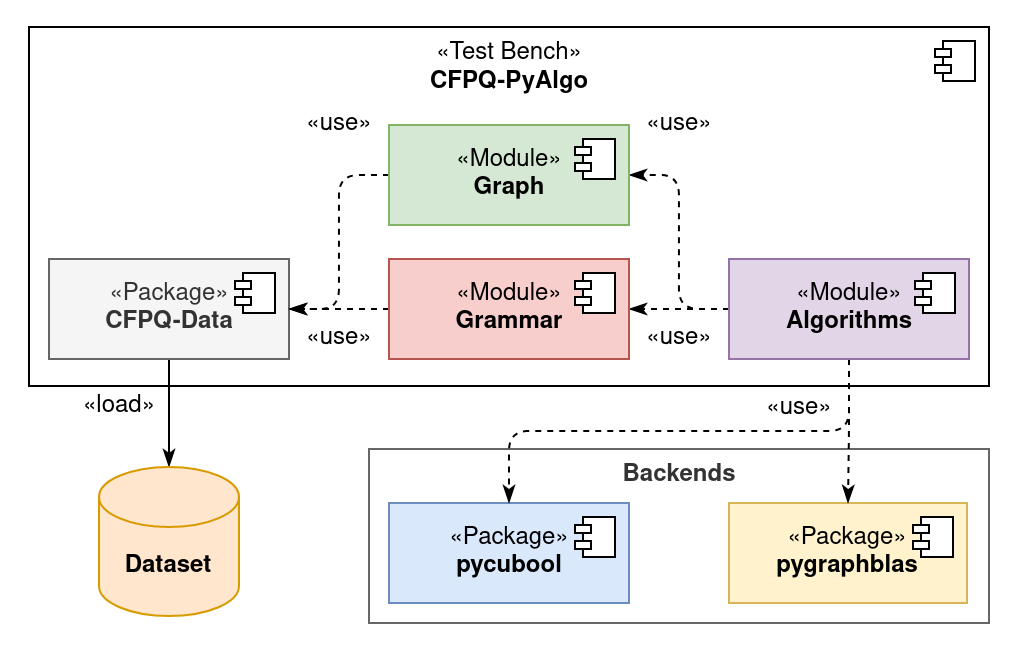
\includegraphics[width=0.9\textwidth]{images/cfpq_pyalgo.png}
    \caption{Архитектура стенда для тестирования алгоритмов}
    \label{fig:cfpq_py_algo}
\end{figure}

В инфраструктуре уже доступны базовые реализации алгоритма Рустама Азимова~\cite{inproceedings:matrix_cfpq} и алгоритма на основе тензорного произведения для вычислений на CPU. 
В качестве основы эти реализации используют пакет \textbf{pygraphblas}, который предоставляет доступ к примитивам разреженной линейной алгебры из стандарта GraphBLAS API~\cite{paper:graphblas_foundations} и его эталонной реализации SuiteSparse~\cite{article:suite_sparse_for_graph_problems}. 
Данные реализации алгоритмов также используются для проведения экспериментального исследования.






\section{Evaluation}

The goal of this evaluation is to investigate the applicability of the proposed algorithm to both regular and context-free path querying.
We measured the execution time of the index creation which solves the reachability problem for both kinds of queries.
The execution time for CFPQ was compared with the Azimov's algorithm for CFPQ reachability.
We also investigated the practical applicability of paths extraction algorithm to both regular and context-free path queries.

For evaluation, we used a PC with Ubuntu 18.04 installed.
It has Intel core i7-6700 CPU, 3.4GHz, and DDR4 64Gb RAM.
We only measure the execution time of the algorithms themselves, thus we assume an input graph is loaded into RAM in the form of its adjacency matrix in the sparse format.
Note, that the time needed to load an input graph into the RAM is excluded from the time measurements.

\subsection{RPQ Evaluation}

To investigate the applicability of the proposed algorithm for regular path querying we gathered a dataset which consists of both real-world and synthetically generated graphs.
We generated the queries from the most popular RPQ templates.

\subsubsection{Dataset}

We gathered several graphs which represent real-world data from different areas and are frequently used for evaluation of the graph querying algorithms.
Namely, the dataset consists of three parts.
The first part is the set of LUBM graphs\footnote{Lehigh University Benchmark (LUBM) web page: \url{http://swat.cse.lehigh.edu/projects/lubm/}. Access date: 07.07.2020.}~\citep{10.1016/j.websem.2005.06.005} which have different numbers of vertices.
The second one is the set of graphs from Uniprot database\footnote{Universal Protein Resource (UniProt) web page: \url{https://www.uniprot.org/}. All files used can be downloaded via the link: \url{ftp://ftp.uniprot.org/pub/databases/uniprot/current_release/rdf/}. Access date: 07.07.2020.}: \textit{proteomes}, \textit{taxonomy} and \textit{uniprotkb}.
The~last part consists of the RDF files \textit{mappingbased\_properties} from DBpedia\footnote{DBpedia project web site: \url{https://wiki.dbpedia.org/}. Access date: 07.07.2020.} and \textit{geospecies}\footnote{The Geospecies RDF: \url{https://old.datahub.io/dataset/geospecies}. Access date: 07.07.2020.}.
A brief description of the graphs in the dataset is presented in Table~\ref{tbl:graphs_for_rpq}.

\begin{table}
    \centering
\caption{Graphs for RPQ evaluation}
\label{tbl:graphs_for_rpq}
{

\rowcolors{2}{black!2}{black!10}
\begin{tabular}{|l|c|c|}
\hline
Graph & \#V & \#E  \\
\hline
\hline
LUBM1k  & 120 926 & 484 646 \\
LUBM3.5k  & 358 434 & 144 9711 \\
LUBM5.9k  & 596 760 & 2 416 513 \\
LUBM1M   & 1 188 340 & 4 820 728 \\
LUBM1.7M & 1 780 956 & 7 228 358 \\
LUBM2.3M & 2 308 385 & 9 369 511 \\
\hline
Uniprotkb & 6 442 630 & 24 465 430 \\
Proteomes & 4 834 262 & 12 366 973 \\
Taxonomy & 5 728 398 & 14 922 125 \\
\hline
Geospecies & 450 609 & 2 201 532 \\
Mappingbased\_properties & 8 332 233 & 25 346 359 \\
\hline
\end{tabular}
}
\end{table}


Queries for evaluation were generated from the templates for the most popular RPQs, specifically the queries presented in Table 2 in~\cite{Pacaci2020RegularPQ} and in Table 5 in~\cite{Wang2019}.
These query templates are presented in Table~\ref{tbl:queries_templates}.
We generate 10 queries for each template and each graph.
The most frequent relations from the given graph were used as symbols in the query template\footnote{Used generator is available as part of CFPQ\_data project: \url{https://github.com/JetBrains-Research/CFPQ_Data/blob/master/tools/gen_RPQ/gen.py}. Access data: 07.07.2020.}.
We used the same set of queries for all LUBM graphs to investigate scalability of the proposed algorithm.

\begin{table}
    \centering
\caption{Queries templates for RPQ evaluation}
\label{tbl:queries_templates}
{\small
\renewcommand{\arraystretch}{1.2}
\rowcolors{2}{black!2}{black!10}
\begin{tabular}{|c|c||c|c|}
\hline

Name & Query & Name & Query \\
\hline
\hline
$Q_1$   & $a^*$                               & $Q_9^5$    & $(a \mid b \mid c \mid d \mid e)^+$                     \\
$Q_2$   & $a\cdot b^*$                        & $Q_{10}^2$ & $(a \mid b) \cdot c^*$                                  \\
$Q_3$   & $a \cdot b^* \cdot c^*$             & $Q_{10}^3$ & $(a \mid b \mid c)  \cdot d^*$                          \\
$Q_4^2$ & $(a \mid b)^*$                      & $Q_{10}^4$ & $(a \mid b \mid c \mid d)  \cdot e^*$                   \\
$Q_4^3$ & $(a \mid b \mid c)^*$               & $Q_{10}^5$ & $(a \mid b \mid c \mid d \mid e)  \cdot f^*$            \\
$Q_4^4$ & $(a \mid b \mid c \mid d)^*$        & $Q_{10}^2$ & $a \cdot b$                                             \\
$Q_4^5$ & $(a \mid b \mid c \mid d \mid e)^*$ & $Q_{11}^3$ & $a \cdot b \cdot c$                                     \\
$Q_5$   & $a \cdot b^* \cdot c$               & $Q_{11}^4$ & $a \cdot b \cdot c \cdot d$                             \\
$Q_6$   & $a^* \cdot b^*$                     & $Q_{11}^5$ & $a \cdot b \cdot c \cdot d \cdot f$                     \\
$Q_7$   & $a \cdot b \cdot c^*$               & $Q_{12}$   & $(a \cdot b)^+ \mid  (c \cdot d)^+$                     \\
$Q_8$   & $a? \cdot b^*$                      & $Q_{13}$   & $(a \cdot(b \cdot c)^*)^+ \mid  (d \cdot f)^+$          \\
$Q_9^2$ & $(a \mid b)^+$                      & $Q_{14}$   & $(a \cdot b \cdot (c \cdot d)^*)^+  \cdot (e \mid f)^*$ \\
$Q_9^3$ & $(a \mid b \mid c)^+$               & $Q_{15}$   & $(a \mid b)^+ \cdot (c \mid d)^+$                       \\
$Q_9^4$ & $(a \mid b \mid c \mid d)^+$        & $Q_{16}$   & $a \cdot b \cdot (c \mid d \mid e)$                     \\
\hline
\end{tabular}
}
\end{table}


\subsubsection{Results}

We averaged the execution time of index creation over 5 runs for each query.
Index creation time for LUBM graphs set is presented in Figure~\ref{fig:lubm_all_qs}.
We can see that evaluation time depends on the query: there are queries which evaluate in less than 1 second even for the largest graphs ($Q_2$, $Q_5$, $Q_{11}^2$, $Q_{11}^3$), while the worst time is 6.26 seconds ($Q_{14}$).
The execution time of our algorithm is comparable with the recent results for the same graphs and queries implemented on a distributed system over 10 nodes~\citep{Wang2019}, while we use only one node.
We conclude that our algorithm demonstrates reasonable performance to be applied to the real-world data analysis.
%\cho{Note that the accurate comparison of different approaches may be a promising direction of future research.}

\begin{figure}
    \centering
   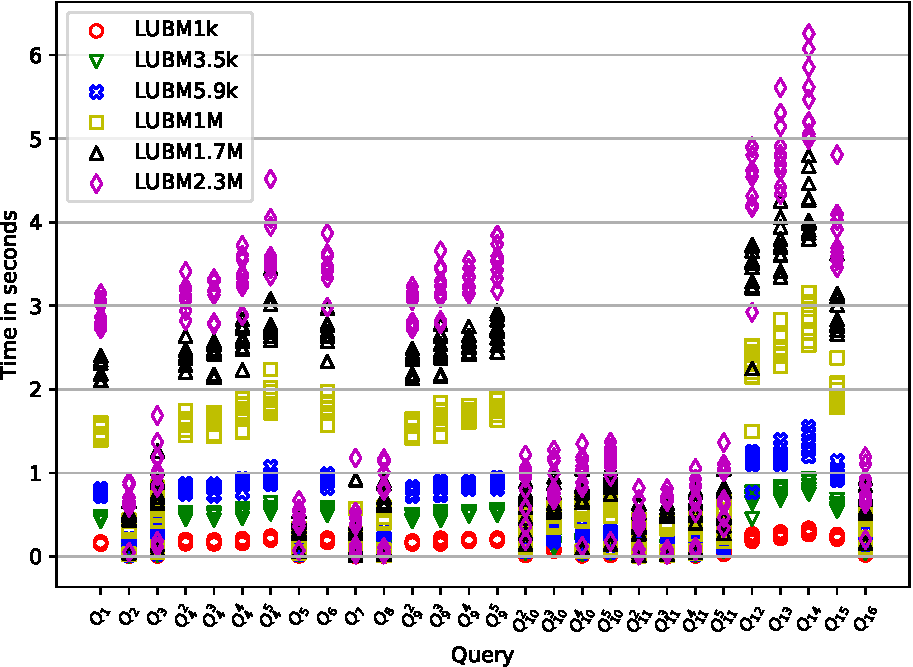
\includegraphics[width=0.6\textwidth]{data/LUBM_all.pdf}
   \caption{Index creation time for LUBM graphs}
   \label{fig:lubm_all_qs}
\end{figure}

Index creation time for each query on the real-world graphs is presented in Figure~\ref{fig:other_all_qs}.
We can see that querying small graphs requires more time than querying bigger graphs in some cases.
For example, conseder $Q_{10}^4$: querying the \textit{geospecies} graph (450k vertices) in some cases requires more time than querying of \textit{mappingbased\_properties} (8.3M vertices) and \textit{taxonomy} (5.7M vertices).
We conclude that the evaluation time depends on the inner structure of a graph.
On the other hand, \textit{taxonomy} querying in many cases requires significantly more time than for other graphs, while \textit{taxonomy} is not the biggest graph.
Finally, in most cases query execution lasts less than 10 seconds, even for bigger graphs, and no query requires more than 52.17 seconds.

\begin{figure}
    \centering
   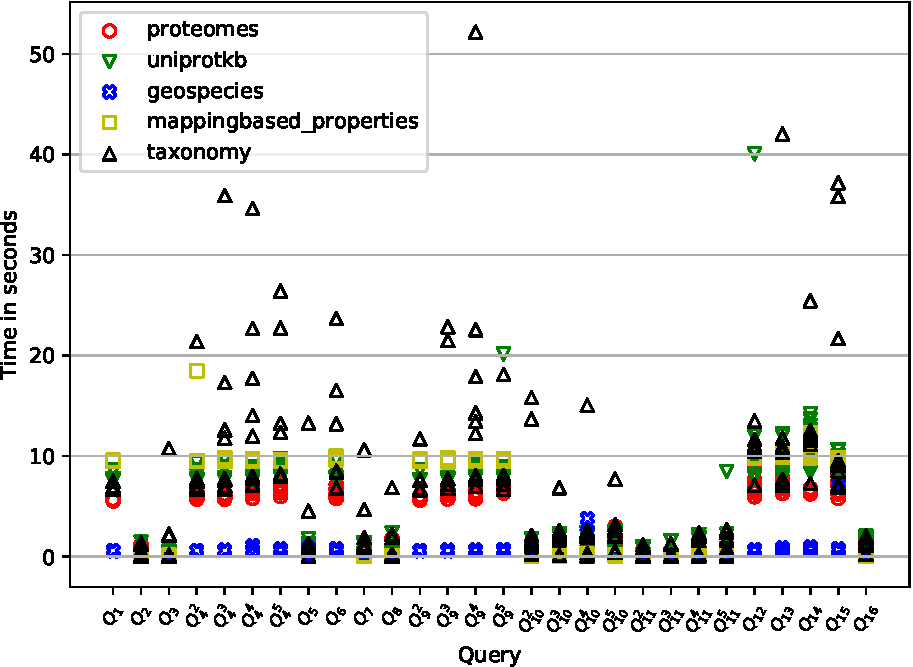
\includegraphics[width=0.6\textwidth]{data/other_all.pdf}
   \caption{Index creation time for real-world RDFs}
   \label{fig:other_all_qs}
\end{figure}

%We evaluate path extraction for queries which result in possibly long paths.
%Long paths usually require many iterations of transitive closure evaluation, thus we used the number of the iterations as a criterion to select the inputs for the evaluation.
%For each selected graph and query we measure paths extraction time for each reachable pair.
%Since the index can be reused from the previous step, we omit the time necessary to create the index.
%We limit by 10 the number of paths to extract.

%In Figures~\ref{fig:geo_tensors_rpq} and~\ref{fig:dbpedia_tensors_rpq} we show the time needed to extract a path of a specific length when only one path was extracted.
%The main observation is that time is linear on the path length, even if a generic path extraction procedure is used.

%\begin{figure}
%     \begin{subfigure}[b]{0.45\textwidth}
%         \centering
%         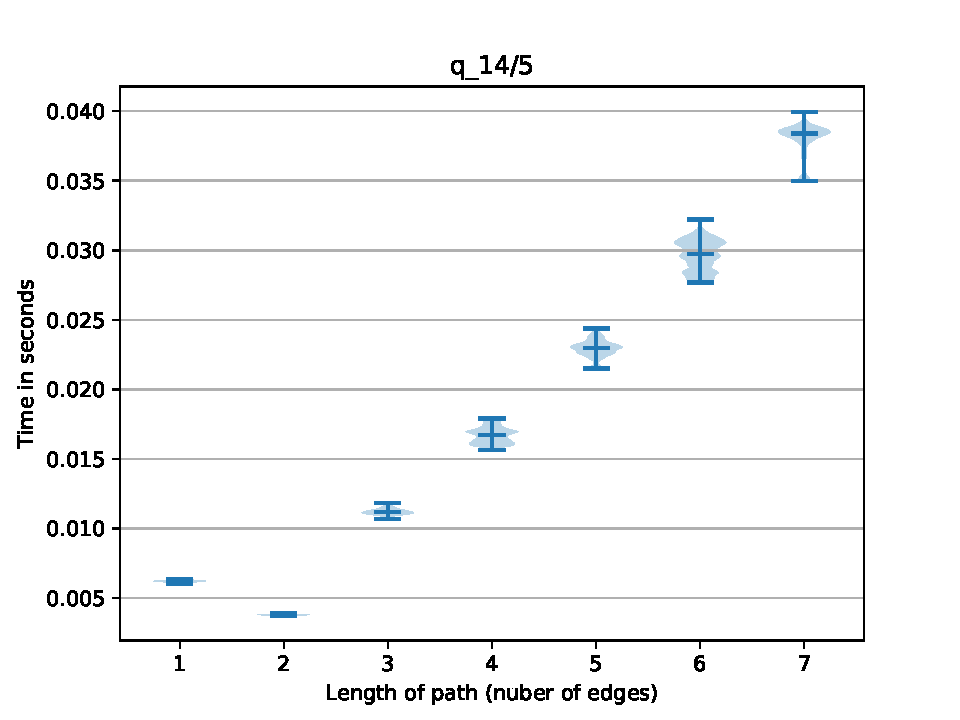
\includegraphics[width=\textwidth]{../paper/data/geo_rpq_single_path/q_14_5.pdf}
%         \caption{\footnotesize \textit{geospecies}, $Q_{14}$}
%         \label{fig:geo_tensors_rpq}
%     \end{subfigure}
%     ~\begin{subfigure}[b]{0.45\textwidth}
%         \centering
%         \includegraphics[width=\textwidth]{../paper/data/CF/Tensor_path/dbpedia_path_tensor.pdf}
%         \caption{\footnotesize \textit{mappingbased\_properties}, $Q_{4}^5$}
%         \label{fig:dbpedia_tensors_rpq}
%     \end{subfigure}\\
%     \begin{subfigure}[b]{0.45\textwidth}
%         \centering
%         \includegraphics[width=\textwidth]{../paper/data/CF/Matrix_CF/geo_path_matrix.pdf}
%         \caption{\footnotesize \textit{geospecies}, \textit{Geo}}
%         \label{fig:geo_matrix_cfpq}
%     \end{subfigure}
%     ~\begin{subfigure}[b]{0.45\textwidth}
%         \centering
%         \includegraphics[width=\textwidth]{../paper/data/CF/Tensor_path/geo_path_tensor.pdf}
%         \caption{\footnotesize \textit{geospecies}, \textit{Geo}}
%         \label{fig:geo_tensors_cfpq}
%     \end{subfigure}\\
%   \caption{Single path extraction for specific graph and query for our solution (\subref{fig:geo_tensors_rpq}, \%subref{fig:dbpedia_tensors_rpq}, \subref{fig:geo_tensors_cfpq}), and Azimov's (\subref{fig:geo_matrix_cfpq})}
%\end{figure}

\subsection{CFPQ Evaluation}

We evaluate the applicability of the proposed algorithm to CFPQ processing over real-world graphs on a number of classic cases and compare them with the Azimov's algorithm.
Currently only a single path version of Azimov's algorithm exists, and we use its implementation using PyGraphBLAS. Note that it is not trivial to compare our results with the state-of-the-art results provided by~\cite{10.1145/3398682.3399163} (Azimov's algorithm) because our algorithm computes significantly more information. While the state-of-the-art solution computes only reachability facts or a single-path semantics, our algorithm computes data necessary to restore all possible paths.

\subsubsection{Dataset}

We use CFPQ\_Data\footnote{CFPQ\_Data is a dataset for CFPQ evaluation which contains both synthetic and real-world data and queries \url{https://github.com/JetBrains-Research/CFPQ\_Data}. Access date: 07.07.2020.} dataset for evaluation.
Namely, we use relatively big RDF files and respective same-generation queries $G_1$~(Eq.~\ref{eqn:g_1}) and $G_2$~(Eq.~\ref{eqn:g_2}) which are used in other works for CFPQ evaluation.
We also use the $Geo$~(Eq.~\ref{eqn:geo}) query provided by~\cite{Kuijpers:2019:ESC:3335783.3335791} for \textit{geospecies} RDF.
Note that we use $\overline{x}$ notation in queries to denote the inverse of $x$ relation and the respective edge.
\begin{align}
\begin{split}
\label{eqn:g_1}
S \to & \overline{\textit{subClassOf}} \ \ S \ \textit{subClasOf} \mid \overline{\textit{type}} \ \ S \ \textit{type}\\   & \mid \overline{\textit{subClassOf}} \ \ \textit{subClasOf} \mid \overline{\textit{type}} \ \textit{type}
\end{split}
\end{align}
\begin{align}
\begin{split}
\label{eqn:g_2}
S \to \overline{\textit{subClassOf}} \ \ S \ \textit{subClasOf} \mid \textit{subClassOf}
\end{split}
\end{align}
\begin{align}
\begin{split}
\label{eqn:geo}
S \to & \textit{broaderTransitive} \ \  S \ \overline{\textit{broaderTransitive}} \\
      & \mid \textit{broaderTransitive} \ \  \overline{\textit{broaderTransitive}}
\end{split}
\end{align}
\begin{align}
\begin{split}
\label{eqn:ma}
S & \to \overline{d} \ V \ d \\
V & \to ((S?) \overline{a})^* (S?) (a (S?))^*
\end{split}
\end{align}

Additionally we evaluate our algorithm on memory aliases analysis problem: a well-known problem which can be reduced to CFPQ~\citep{Zheng:2008:DAA:1328897.1328464}.
To do it, we use some graphs built for different parts of Linux OS kernel (\textit{arch}, \textit{crypto}, \textit{drivers}, \textit{fs}) and the query $MA$~(Eq.~\ref{eqn:ma})~\citep{10.1145/3093336.3037744}.
The detailed data about all the graphs used is presented in Table~\ref{tbl:graphs_for_cfpq}.

{\setlength{\tabcolsep}{0.3em}
\begin{table}
    \centering
{
\caption{Graphs for CFPQ evaluation: \textit{bt} is broaderTransitive, \textit{sco} is subCalssOf}
\label{tbl:graphs_for_cfpq}
\scriptsize
\rowcolors{2}{black!2}{black!10}
\begin{tabular}{|l|c|c|c|c|c|c|c|}
\hline
Graph          & \#V       & \#E        & \#sco & \#type &\#bt & \#a  & \#d \\
\hline
\hline
eclass\_514en  & 239 111    & 523 727    & 90 512    & 72 517    &        ---        & ---  & --- \\
enzyme         & 48 815     & 109 695    & 8 163     & 14 989    &        ---        & ---  & --- \\
geospecies     & 450 609    & 2 201 532  & 0         & 89 062    &        20 867     & ---  & --- \\
go             & 272 770    & 534 311    & 90 512    & 58 483    &        ---        & ---  & --- \\
go-hierarchy   & 45 007     & 980 218    & 490 109   & 0         &        ---        & ---  & --- \\
taxonomy       & 5 728 398  & 14 922 125 & 2 112 637 & 2 508 635 &        ---        & ---  & --- \\
\hline
arch           & 3 448 422  & 5 940 484  &      ---     &  ---   &        ---        & 671 295 & 2 298 947 \\
crypto         & 3 464 970  & 5 976 774  &      ---     &  ---   &        ---        & 678 408 & 2 309 979 \\
drivers        & 4 273 803  & 7 415 538  &      ---     &  ---   &        ---        & 858 568 & 2 849 201 \\
fs             & 4 177 416  & 7 218 746  &      ---     &  ---   &        ---        & 824 430 & 2 784 943 \\
\hline
\end{tabular}
}
\end{table}
}
\subsubsection{Results}

We averaged the index creation time over 5 runs for both single-path Azimov's algorithm (\textbf{Mtx}) and the proposed algorithm (\textbf{Tns}) (see Table~\ref{tbl:CFPQ_index}).

{\setlength{\tabcolsep}{0.2em}
  \begin{table}
    \centering
    \caption{CFPQ evaluation results, time is measured in seconds}
    \label{tbl:CFPQ_index}
    \rowcolors{4}{black!2}{black!10}
    \small
    \begin{tabular}{| l | c | c | c | c | c | c | c | c |}
      \hline

      \multirow{2}{*}{Name}  & \multicolumn{2}{c|}{$G_1$} & \multicolumn{2}{c|}{$G_2$} & \multicolumn{2}{c|}{\textit{Geo}} & \multicolumn{2}{c|}{\textit{MA}}\\
      \cline{2-9}
                      & Tns    & Mtx    & Tns  & Mtx  & Tns   & Mtx   & Tns     & Mtx \\
      \hline
      \hline
      eclass\_514en   & 0.24   & 0.27   & 0.25 & 0.26 & ---   & ---   & ---     & ---\\
      enzyme          & 0.03   & 0.04   & 0.02 & 0.01 & ---   & ---   & ---     & ---\\
      geospecies      & 0.08   & 0.06   & $0^{*}$ & 0.01 & 26.12 & 16.58 & ---     & ---\\
      go-hierarchy    & 0.16   & 1.43   & 0.23 & 0.86 & ---   & ---   & ---     & ---\\
      go              & 1.56   & 1.74   & 1.21 & 1.14 & ---   & ---   & ---     & ---\\
      pathways        & 0.01   & 0.01   & 0.01 & 0.01 & ---   & ---   & ---     & ---\\
      taxonomy        & 4.81   & 2.71   & 3.75 & 1.56 & ---   & ---   & ---     & ---\\
      \hline
      arch            & ---    & ---    & ---  & ---  & ---   & ---   & 262.45  & 195.51  \\
      crypto          & ---    & ---    & ---  & ---  & ---   & ---   & 267.52  & 195.54  \\
      drivers         & ---    & ---    & ---  & ---  & ---   & ---   & 1309.57 & 1050.78 \\
      fs              & ---    & ---    & ---  & ---  & ---   & ---   & 470.49  & 370.73  \\
      \hline
    \end{tabular}
  \end{table}
}

Best to our knowledge, the proposed algorithm is the first algorithm that provides information about all paths of interest (Azimov's algorithm computes information about only one path).
The direct comparison with other solutions is impossible, and we just estimate the running time of our algorithm for a small number of cases.
Namely, we extract all paths with length not greater than 20 edges between all pairs of vertices from indeces created for graphs \textit{go} and \textit{eclass\_514en} and query $G_1$.
Paths extraction for one pair of vertices requires 2.64 seconds averaged over all pairs for \textit{go} graph. The~maximal time is 4699 seconds and 217737 paths were extracted during this time. The average number of paths between two vertices is 184.
For \textit{eclass\_514en} paths extraction for one pair of vertices requires 1.27 seconds averaged over all pairs. The~maximal time is 8.04 seconds and only one path is extracted during this time. The average number of paths between two vertices is 3.
We can see that paths can be extracted in a reasonable time, but a detailed analysis of paths extraction algorithm performance depends on graphs structure.

%Comparison of paths extraction is presented in Figures~\ref{fig:geo_matrix_cfpq} and~\ref{fig:geo_tensors_cfpq}.
%While both methods demonstrate linear time on the length of the extracted path, our generic solution is more than 1000 times slower than Azimov's single path extraction procedure.
%We conclude that current generic all-path extraction procedure is not optimal for single path extraction.

\subsection{Conclusion}

We conclude that the proposed algorithm is applicable to real-world data processing: the algorithm allows one to solve both the reachability problem and to extract paths of interest in a reasonable time even using naive implementation.
While index creation time (reachability query evaluation) is comparable with other existing solutions, paths extraction procedure should be improved in the future. However, the state-of-the-art solution computes only reachability facts or a single-path semantics, whereas our algorithm computes data necessary to restore all possible paths (all-paths semantics).
Finally, a detailed comparison of the proposed solution with other algorithms for CFPQ and RPQ is required.

To summarize the overall evaluation, the proposed algorithm is applicable to both RPQ and CFPQ over real-world graphs.
Thus, the proposed solution is a promising unified algorithm for both RPQ and CFPQ evaluation.

\section{Conclusion}

Conclusion, current state, results.

Future work. Library extension up to full GraphBLAS API implementation.

LaGraph on F\# .NET.

Evaluation. Comparison with other implementations on different devices.
Manual implementation versus translation.  

Another direction of future work is Brahma.FSharp improvements. 
First of all, it is necessary to support discriminated unions to make it possible to express custom semirings such as \texttt{Min-Plus}, as presented in listing~\ref{lst_example}. 

Also, it is necessary to add high-level abstractions for asynchronous programming, and for multi-GPU programming.
Such mechanisms can be naturally expressed in F\# with native primitives for asynchronous programming.

fusion and other optimizations.

% \section{Эксперимент}
% Как мы проверяем, что  всё удачно получилось

% \subsection{Условия эксперимента}
% Железо (если актуально); входные данные, на которых проверяем наш подход; почему мы выбрали именно эти тесты

% \subsection{Исследовательские вопросы (Research questions)}
% Надо сформулировать то, чего мы хотели бы добиться работой (2 штуки будет хорошо):

% \begin{itemize}
% \item Хотим алгоритм, который лучше вот таких-то остальных
% \item Если в подходе можно включать/выключать составляющие, то насколько существенно каждая составляющая влияет на улучшения
% \item Если у нас строится приближение каких-то штук, то на сколько точными будут эти приближения
% \item и т.п.
% \end{itemize}

% \subsection{Метрики}

% Как мы сравниваем, что результаты двух подходов лучше или хуже
% \begin{itemize}
% \item Производительность
% \item Строчки кода
% \item Как часто алгоритм "угадывает" правильную классификацию входа
% \end{itemize}

% Иногда метрики вырожденные (да/нет), это не очень хорошо, но если в области исследований так принято, то ладно.

% \subsection{Результаты}
% Результаты понятно что такое. Тут всякие таблицы и графики

% В этом разделе надо также коснуться Research Questions.

% \subsubsection{RQ1} Пояснения
% \subsubsection{RQ2} Пояснения

% \subsection{Обсуждение результатов}

% Чуть более неформальное обсуждение, то, что сделано. Например, почему метод работает лучше остальных? Или, что делать со случаями, когда метод классифицирует вход некорректно.

% \section{Применение того, что сделано на практике (опциональный)}

% Если применение в лоб не работает, потому что всё изложено чуть более сжато и теоретично, надо рассказать тонкости и правильный метод применения результатов. 

% \section{Угрозы нарушения корректности (опциональный)}

% Если основная заслуга метода, это то, что он дает лучшие цифры, то стоит сказать, где мы могли облажаться, когда проводили численные замеры. 

% \section{Заключение}

% Кратко, что было сделано. Также здесь стоит писать задачи на будущее.

% \textbf{Для курсовых/дипломов.} Также стоит сделать список результатов, который будет 1 к одному соответствовать задачам из раздела~\ref{sec:task}.

% \begin{itemize}
% \item Результат к задаче 1 
% \item Результат к задаче 2
% \item и т.д.
% \end{itemize}

% \nocite{*}
\setmonofont[Mapping=tex-text]{CMU Typewriter Text}
\bibliographystyle{ugost2008ls}
\bibliography{kronecker_cfpq_gpu_diploma}

\end{document}